\documentclass[11pt]{article}

 
\usepackage{graphics}
\usepackage{graphicx}
\usepackage{pstricks}

\title{\textsf{molsim} tutorial}
\author{J.S. Hansen}
\date{Februaray 2022, v. 0.9}
  
\begin{document}

\maketitle

\section{Introduction}

\textsf{molsim} is a GNU Octave/Matlab toolbox for molecular dynamics simulation
library. \textsf{molsim} supports simulations of
\begin{itemize}
\item standard Lennard-Jones systems,
\item molecular systems with bond, angle, and torsion potentials, 
\item confined flow systems, eg., Couette and Poiseuille flows,
\item charged systems using shifted force and Wolf methods,
\item dissipative particle dynamics systems,
\item and more \ldots
\end{itemize}
The package also supports a series of run-time sampling functionalities.

\bigskip
\noindent \textsf{molsim} is basically a wrapper for the \textsf{seplib}
library, which is a light-weight flexible molecular dynamics simulation library
written in ISO-C99. The library is CPU-based and offers shared memory
parallisation; this parallisaton is supported by the \textsf{molsim}
package. The algorithms used in \textsf{seplib} is based on the books by Allen
\& Tildesley, Rapaport, Frenkel \& Smith, and R. Sadus, see
Ref. \cite{seplib:books}.

\bigskip
\noindent In this text
\begin{verbatim}
>> 
\end{verbatim}
symbolises the GNU Octave/Matlab command prompt. This 
\begin{verbatim}
$ 
\end{verbatim}
symbolises the shell prompt.

\section{Installation}
\subsection{GNU Octave}
GNU Octave's package manager offers a very easy installation. From

\begin{verbatim}
https://github.com/jesperschmidthansen/molsim/
\end{verbatim}

\noindent download and save the current release
\verb!molsim-<version>.tar.gz! in a directory of your choice. Start GNU
Octave and if needed change directory to the directory where the file is saved.

\noindent Then type
\begin{verbatim}
>> pkg install molsim-<version>.tar.gz 
\end{verbatim}
to install the package. Check contact by
\begin{verbatim}
>> molsim('hello')
Hello. 
\end{verbatim}
In case this fails, check the path where \textsf{molsim} is install by
\begin{verbatim}
>> pkg list molsim
\end{verbatim}
If the path is not in your GNU Octave search path add this using the
\verb!addpath! command.

\subsection{Matlab}
From
\begin{verbatim}
https://github.com/jesperschmidthansen/seplib/
\end{verbatim}
\noindent download and save the current release \verb!seplib-<version>.tar.gz!
in a directory of your choice. Unpack, configure and build the library
\begin{verbatim}
$ tar zxvf seplib-<version>.tar.gz
$ cd seplib
$ ./configure
$ make
$ cd octave
\end{verbatim}
To build the \textsf{mex}-file enter Matlab
\begin{verbatim}
$ matlab -nodesktop
\end{verbatim}
Then build the 
\begin{verbatim}
>> buildmex
\end{verbatim}
Depending on the system this will build a \textsf{molsim.mex<archtype>}
file. You can copy this file to a directory in your Matlab search path.

\section{First quick example: The Lennard-Jones liquid}
Listing 1 shows the simplest script simulating a standard Lennard-Jones (LJ)
system in the micro-canonical ensemble where number of particles, volume, and
total energy is conserved. 

\bigskip

\noindent \textbf{Listing 1}
\begin{verbatim}
% Specify the LJ paramters
cutoff = 2.5; epsilon = 1.0; sigma = 1.0; aw=1.0;

% Set init. position and velocities 10x10x10 particles 
% in box with lengths 12x12x12. Velocities set to default. 
% Configuration stored in start.xyz. 
molsim('set', 'lattice', [10 10 10], [12 12 12]);

% Load the configuration file
molsim('load', 'xyz', 'start.xyz');

% Main mol. simulation loop - 10 thousand time steps
for n=1:10000

  % Reset everything
  molsim('reset');

  % Calculate force between particles of type A (default type)
  molsim('calcforce', 'lj', 'AA', cutoff, sigma, epsilon, aw);

  % Integrate forward in time - use leapfrog alogrithm
  molsim('integrate', 'leapfrog');
 
end

% Free memory allocated
molsim('clear');
\end{verbatim}
---

\noindent Listing 1 is not very useful as no information is printed or saved. Inside the
main loop you can add the command
\begin{verbatim}
if rem(n,100)==0
  molsim('print');
end
\end{verbatim}
to print current iteration number, potential energy per particle, kinetic energy
per particle, total energy per particle, kinetic temperature, and total momentum
to screen every 100 time step.

Information can also be stored into variables for further analysis. For example,
to get the system energies and pressure
\begin{verbatim}
[ekin, epot] = molsim('get', 'energies');
press = molsim('get', 'pressure');
\end{verbatim}
and particle positions and velocities
\begin{verbatim}
x = molsim('get', 'positions');
v = molsim('get', 'velocities');
\end{verbatim}

\bigskip

\noindent In general, the \verb!molsim! interface is on the form
\begin{verbatim}
molsim(ACTION, SPECIFIER, ARGUMENTS);
\end{verbatim}
where the action can be \verb!get!, \verb!calcforce!, and so on, the specifier
is a specification for the action, eg., \verb!lj! specifýing that the force is a
pair-wise Lennard-Jones force, and arguments are the arguments for the
specifier.

\subsection{NVT and NPT simulations}
Often you will not perform simulations in the microcanonical ensemble, but under
a desired temperature and/or pressure. One way to achieve this with
\verb!molsim! is to use simple relaxation algorithms. To simulate at
temperature, say 2.2, you call the action \verb!'thermostate'! with specifier
\verb!'relax'! after the integration step
\begin{verbatim}
molsim('thermostate', 'relax', 2.2, 0.01);
\end{verbatim}
The last argument is the relaxation parameter; the higher value the faster
relaxation. Notice that too large values makes the system unrealistically
stiff. The best value is optimed via trail-and-error.

To simulate at pressure, say 0.9, you call the action \verb!'barostate'! after
the integration step,
\begin{verbatim}
molsim('barostate', 'relax', 0.9, 0.01);
\end{verbatim}
The choice of relaxation parameter is again a matter of the system. You can use
the two relaxation actions in the same simulation mimicking an NPT system. The
barostate works by changing the system box length in the $z$-direction only
(an-isotropic scaling); this is practical when doing sampling as two directions
are fixed.

\section{The \textsf{molsim} force field}
\textsf{molsim} supports simulations of confined, charged, and molecular
systems. In general, the interaction \textsf{molsim} force field is defined from
the potential functional form
\begin{equation}
  U(\mathbf{r}_i, r_{ij}, \ldots)
  =  U_\mathrm{lattice} + U_\mathrm{vWaals} + U_{\mathrm{coloumb}} +
  U_\mathrm{bonds} + U_\mathrm{angles} + 
  U_\mathrm{dihedrals}
\end{equation}
The first term allows for a simulation of a fictitious fixed crystal
arrangement, where the particles/atoms are tethered around a pre-set lattice
site. The potential function is a harmonic spring type
\begin{equation}
  U_\mathrm{lattice} =
  \sum_\mathrm{sites} \frac{1}{2}k_0 (\mathbf{r}_i - \mathbf{r}_0)^2
\end{equation}
where $k_0$ is the spring constant, $\mathbf{r}_i$ is the position of
particle/atom $i$, and $\mathbf{r}_0$ is the lattice site. The default
lattice site positions are the initial particle positions.

The short ranged van der Waals pair interaction is given via the standard
Lennard-Jones potential
\begin{equation}
  U_\mathrm{vWaals} =  \sum_{i,j \, \mathrm{pairs}}
  4\epsilon\left[\left(\frac{\sigma}{r_{ij}}\right)^{12} - a_w
    \left(\frac{\sigma}{r_{ij}}\right)^{6}\right] \, .
\end{equation}
Here $r_{ij}$ is the particle distance, $\epsilon$ and $\sigma$ define the
characteristic energy and length scales. The parameter $a_w$ determines the
weight of the attractive second term in the potential function.

The Coulomb potential is 
\begin{equation}
  U_{\mathrm{coloumb}} = \sum_{i,j \, \mathrm{pairs}}\frac{q_iq_j}{r_{ij}} \, .
\end{equation}
This long ranged interaction is evaluated using approximative shifted-force or
Wolf methods; this can be specified. These two implementations do not apply to
confined systems.

Particle bonds are model via the harmonic spring potential
\begin{equation}
  U_{\mathrm{bonds}} =\sum_{\mathrm{bonds}} \frac{1}{2} k_{s}(r_{ij} - l_0)^2
\end{equation}
$k_s$ is the spring constant and $l_0$ is the zero force bond length. Note,
currently \textsf{molsim} does not support rigid bonds.

The angle potential is the cosine squared potential
\begin{equation}
  U_{\mathrm{angles}}=\frac{1}{2}\sum_{\mathrm{angles}} k_{\theta} (\cos(\theta) - \cos(\theta_0))^2 \, ,
\end{equation}
where $k_\theta$ is the force amplitude, and the zero-force angle
$\theta_0$. See Fig. \ref{fig:diheadral} for the angle definition.

\begin{figure}[h]
  \begin{center}
    \includegraphics[scale=.7]{diheadral.pdf}
  \caption{
    \label{fig:dihedral}
    sds
  }
  \end{center}
\end{figure}

Finally, the dihedral angle potential is the Ryckaert-Belleman potential 
\begin{equation}
  U_\mathrm{dihedral}=\sum_{\mathrm{dihedrals}} \sum_{n=0}^5 c_n
  \cos^n(\pi-\phi)
   \, . 
\end{equation}
Here $c_n$ are the six Ryckaert-Belleman coefficients, and $\phi$ is the
dihedral angle, see Fig. \ref{fig:dihedral}. Two illustrative 
examples are when $c_n = 0$ except for $n=1$:
\begin{enumerate}
\item If $c_1 > 0$ then the minimum energy dihedral angle is $\phi = 0$; this is
  illustrated in the right-hand figure in Fig. \ref{fig:dihedral} with dihedral
  defined by the 1-2-3-5 bonds. Useful for closed molecular ring structures.
\item If $c_1 < 0$ then the minimum dihedral angle is $\phi = \pi$; this is
  illustrated in the right-hand figure in Fig. \ref{fig:dihedral} with
  dihedral defined by the 1-2-3-4 bonds. Useful for branched molecular
  structures. 
\end{enumerate}
Below a more complex example is given.

Importantly, you can have different types of particles with different charges,
different bonds, angles, and dihedrals, all determined from the interaction
parameters. It is thus possible to simulate mixtures, highly complex molecules,
etc. 

\section{Molecular systems: Toluene and water}

\section{Dissipative particle dynamics (DPD)}
\section{Sampling}
\section{The two parallisation paradigms}

\end{document}
